\section{Technical Method Details}
\subsection{Landmarks and Baseline}
Images are processed with MediaPipe Hand Landmarker. The intended extraction settings are IMAGE mode, up to two hands, and detection/presence thresholds of 0.5; only exactly one accepted hand is used. Historical records contain the MediaPipe version and landmarks, but not the threshold values. Thus default-setting provenance cannot be independently confirmed for the historical cache. We preserve these landmarks for all comparisons rather than rerun detection differently per model.

The Shin implementation follows the paper's pair list: 190 pairwise distance features and 630 axis-direction features, for 820 features overall. Distance features are normalized per image; direction features are cosine-based encodings of inter-landmark vectors relative to axes. The local implementation preserves the paper's listed pair exclusions. Features use image landmarks for the baseline and estimated world landmarks for the added hand geometry.

\begin{figure}[t]
\centering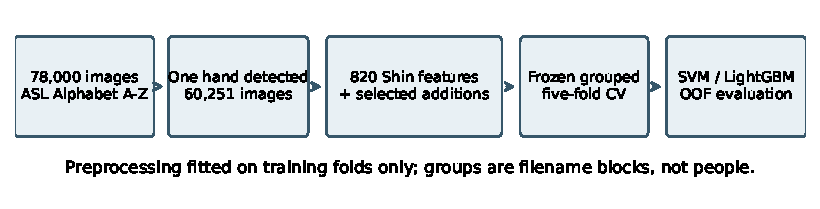
\includegraphics[width=\linewidth]{figures/pipeline.pdf}
\caption{Evaluation pipeline. Every compared model uses the same 60,251 accepted images and frozen outer folds. Detection coverage and conditional classification accuracy are separate quantities.}
\label{fig:pipeline}
\end{figure}

\subsection{Interpretable Additions}
For consecutive landmarks $a,b,c$, an interior bending angle is
\begin{equation}
\theta(a,b,c)=\arccos\frac{(a-b)^\top(c-b)}{\|a-b\|\,\|c-b\|}\frac{180}{\pi}.
\end{equation}
A straight joint approaches $180^\circ$. We use thumb MCP/IP and MCP/PIP/DIP for the other four fingers: 14 interior angles. A signed thumb-MCP deviation adds a fifteenth measurement. MCP measurements are landmark-based proxies, not calibrated clinical joint measurements. The retained phrase ``angles'' below always means all 15 additions, not a fourteenth-angle-only experiment.

Categorical features encode bent, partly bent and extended joints; a binary B-shaped/non-B-shaped thumb MCP; and spread, suspected crossing and thumb contact relations. An unknown state is retained. Thresholds are fixed across folds. Non-thumb flexion uses $\leq130^\circ$ for bent and $\geq150^\circ$ for extended, with intermediate values partly bent. Finger spread requires separation in approximately the same plane; splaying is allowed. Crossing and contact are geometric proxies and remain sensitive to occlusion and depth estimates.

The workbook gives the allowed categories for each letter. A slash means a set of acceptable alternatives, not a new combined class. One-hot measured categories yield 70 inputs. For each candidate letter $\ell$, a compatibility score averages the proportion of specified workbook cells whose allowed set contains the measured category. This produces 26 scores. All 26 are computed for every image without accessing its true label. A fixed 49-cell slash-relaxation proposal was developed in earlier exploratory work; its changes are preserved separately from the user's original workbook. This reference design was not nested within the later evaluation.

\subsection{Models, Scaling and Weighting}
The primary SVM uses an RBF kernel, $C=10$, \texttt{gamma=scale} and balanced class weights. This differs from the paper-profile $C=1000$ with no class balancing. Its soft-margin objective balances margin size against weighted classification slack. For input blocks $z_b$ and weights $w_b$, the RBF similarity is
\begin{equation}
K(x,x')=\exp\!\left(-\gamma\sum_b w_b^2\|z_b(x)-z_b(x')\|^2\right).
\end{equation}
For each binary letter pair, the kernel SVM minimizes the regularized hinge loss
\[
\frac12\|w\|^2+C\sum_i\omega_i\max(0,1-y_i(w^\top\phi(x_i)+b)),
\]
where $y_i\in\{-1,1\}$, $\phi$ is the kernel feature mapping and $\omega_i$ combines class and sample weights. The multiclass decision uses pairwise voting. LightGBM instead optimizes multiclass log loss with tree-complexity control. These objectives were not modified to prefer individual letters.

Thus a multiplier of two contributes a factor of four inside the squared distance, while \texttt{gamma=scale} also changes with the input variance. Angle median imputation and standardization are fitted within each training fold; baseline descriptors and categorical/compatibility values pass through unchanged. No missing angles occurred in the retained cache.

LightGBM optimizes multiclass log loss through boosted trees, using 100 estimators, 31 leaves, learning rate 0.1 and minimum child size 20. Its fixed project profile is not a replication of the paper's tuned LightGBM settings. Group weighting searches use inner-fold macro-F1, breaking ties by accuracy. They make one coordinate pass, not an exhaustive global search.


\section{Earlier Experimental Settings and Results}
\subsection{Implementation and Experimental Sequence}
Experiments use Python 3.12, MediaPipe 0.10.35, scikit-learn 1.8.0 and LightGBM 4.7.0. An earlier three-fold pilot tested 81 continuous/binary finger-geometry descriptors, alone and combined with baseline descriptors. This differs from the later 70-column categorical encoding and is not mixed into the five-fold table. The pilot feature-only model reached 93.71\% mean fold accuracy, versus 97.43\% for the baseline; combining them did not improve the baseline. It did not isolate replacement of only the 190 distances while retaining all 630 directions.

The main sequence compares the 820 baseline, all 111 additions (931 total), then isolated angle and compatibility-score additions. Grouped permutation analysis shuffles whole related columns jointly on held-out data, five repeats with at most 100 images per letter per fold. Ablations remove a block and refit. These analyses share the fixed full-input model and should not be interpreted as interchangeable measures.

Block weighting tries 0.25, 0.5, 1 and 2. Targeted index MCP/PIP/DIP weighting tries 0.5, 1 and 2. Both use five outer and three inner group folds, with inner training and validation capped at 150 images per letter for cost. The final outer fits use all outer-training images. This is bounded exploratory tuning, not exhaustive hyperparameter optimization.


\subsection{Isolated SVM and LightGBM results}
\begin{table}[h]\centering\caption{Detailed original isolated comparison; these results concern matched accepted images.}
\begin{tabular}{lrrrrr}\toprule
Representation & Inputs & SVM acc. (\%) & SVM macro-F1 & LGBM acc. (\%) & LGBM macro-F1\\\midrule
\tableinput result_rows.tex
\bottomrule\end{tabular}\end{table}

The full 931-input SVM scored 97.62826\% and LightGBM 97.16353\%. Removing categorical one-hot columns produced 97.74444\% for SVM, matching the isolated angle-plus-workbook model. In the grouped permutation analysis, shuffling angles reduced SVM macro-F1 by 0.570 percentage points, compared with 0.049 for categories and 0.008 for workbook compatibility scores. For LightGBM these drops were 0.031 and 0.200 for angles and compatibility scores. These overlapping reliance measures are not additive or causal.

The source article reports 87.60\% ASL Alphabet combined-feature SVM accuracy, no matching F1 metric, and a held-out evaluation with tuning rather than this filtered grouped protocol. It also states 780,000 images inconsistently with 26 times 3,000; the actual inventory is 78,000. The local paper-profile SVM ($C=1000$, no balancing) reached 97.66145\%; changing this setting alone does not reconcile the protocols. Detection, data selection and split differences have not been isolated experimentally.
